\chapter{L'applicazione lato utente}
Nella prima parte di questo capitolo, vengono illustrati i requisiti di sistema che hanno guidato lo sviluppo dell'intera applicazione. Mentre nella parte finale verranno mostrati i task principali e le relative schermate dell'interfaccia realizzata con il framework Ratchet (vedi \ref{ratchet}).
\section{Requisiti di sistema}
La stesura dei requisiti di sistema è un processo imprenscindibile per la progettazione, nel nostro caso è il risultato di un processo iterativo basato sulla valutazione di un esperto.\\
I requisiti sono divisi in:
\begin{itemize}
\item \textbf{Requisiti funzionali} indicano quello che il sistema deve fare
\item \textbf{Requisiti non funzionali} vincoli sul sistema e il suo sviluppo
\end{itemize}
 
 \subsection{Requisiti funzionali}

\begin{enumerate}
\item Interazione mappa
  \begin{itemize}
     \item\textit{Identificativo:} RF-1
  \item\textit{Descrizione:} Il sistema deve permettere all’utente di interagire con la mappa, compiendo le azioni basilari quali: zoom In, zoom Out, CCW (Change Center View), click.
  \end{itemize}
  \newpage
\item Impostazione POI
  \begin{itemize}
  \item\textit{Identificativo:} RF-2
  \item\textit{Descrizione:} Il sistema deve permettere all’utente di impostare una specifica porzione di mappa come un POI (point of interest).
  \item\textit{Razionale:} In questo modo l’utente può applicare un filtro sulla mappa (vedi RF-7)  e visualizzare rapidamente lo status dei luoghi d’interesse.
  \end{itemize}
  
\item Impostazione FOI
  \begin{itemize}
  \item\textit{Identificativo:} RF-3
  \item\textit{Descrizione:} Il sistema deve permettere all’utente di impostare altri utenti del sistema come FOI (family of interest).
  \item\textit{Razionale:} l’utente può in questo modo applicare un filtro (vedi RF-7) e visualizzare in modo rapido lo status delle persone d’interesse.
  \end{itemize}
  
  \item Segnalazione evento
  \begin{itemize}
  \item\textit{Identificativo:} RF-4
  \item\textit{Descrizione:} l’utente deve poter segnalare la posizione di un certo evento (vedi RNF-1). 
La procedura standard di segnalazione deve avvenire sia cliccando su un punto della mappa sia tramite una schermata dedicata.
Nel caso di rete congestionata o assente il sistema deve provvedere alla bufferizzazione delle richieste e avvisare di tale situazione l’utente stesso.
  \item\textit{Razionale:} In questo modo gli utenti contribuiscono all’aggiornamento dello status generale del territorio colpito.
  \end{itemize}
  
   \item Aggiornamento status
  \begin{itemize}
  \item\textit{Identificativo:} RF-5
  \item\textit{Descrizione:} L’utente può cambiare il suo status (vedi RNF-4). Il sistema quindi deve comunicare immediatamente al server tale aggiornamento.
  \item\textit{Razionale:} In questo modo gli utenti contribuiscono a fornire informazioni dinamiche sul territorio colpito e su se stessi.
  \end{itemize}
  
  \item Trusty data
  \begin{itemize}
  \item\textit{Identificativo:} RF-6
  \item\textit{Descrizione:} Il sistema deve informare l’utente sul grado di aggiornamento delle informazioni visualizzate, ovvero:
    \begin{itemize}
    \item Eventi
    \item Status dei POI
    \item Status dei FOI
    \item mappe offline
    \end{itemize}
   L’attendibilità degli eventi è data dal numero di segnalazioni di tale evento nella relativa cella (vedi RNF-1) e dall’orario in cui è stata generata l’ultima    segnalazione.
   \item\textit{ Razionale:} Nel contesto d’uso, la rete potrebbe collassare o più semplicemente gli utenti potrebbero non utilizzare il sistema per un certo periodo, in questo modo si garantisce la totale trasparenza delle informazioni fornite.
  \end{itemize}
  
  \item Filtra mappa
  \begin{itemize}
  \item\textit{Identificativo:} RF-7
  \item\textit{Descrizione:} Il sistema deve permettere all’utente di filtrare le informazioni visibili sulla mappa in base a:
    \begin{itemize}
    \item propri POI
    \item tipo eventi
    \item propri FOI
    \end{itemize}
   \item\textit{Razionale:} La mappa visualizzata dall’utente potrebbe contenere un numero elevato di informazioni.
  \end{itemize}
  
    \item Modalità offline
  \begin{itemize}
  \item\textit{Identificativo:} RF-8
  \item\textit{Descrizione:} Il sistema deve salvare porzioni di mappa visualizzate dall’utente attraverso l’interazione base (vedi RF-1) nella memoria temporale, inoltre l’utente deve poter scaricare una specifica center view su diversi livelli di zoom. Il sistema quindi deve permettere all’utente di utilizzare la modalità offline, in questo caso la rete verrà utilizzata solamente per inviare e ricevere aggiornamenti riguardo:
    \begin{itemize}
    \item POI e NPOI
    \item FOI e NFOI
    \item Eventi
    \end{itemize}
   \item\textit{Razionale:} L’utente potrebbe voler utilizzare la modalità offline per risparmiare dati o per la  pessima connessione
  \end{itemize}
  
   \item Markercluster
  \begin{itemize}
  \item\textit{identificativo:} RF-9
  \item\textit{Descrizione:} Il sistema per livelli di zoom, sufficientemente bassi, deve raggruppare i marker in un unico markercluster; inoltre deve mostrare la quantità di elementi inglobati.
  \end{itemize}
  
    \item Aggiornamento dati persistenti
  \begin{itemize}
  \item\textit{identificativo:} RF-10
  \item\textit{Descrizione:} Il sistema deve periodicamente richiedere al server l’aggiornamento dei dati persistenti (vedi RNF-2).
Inoltre l’utente può richiedere l’aggiornamento in qualsiasi momento
  \end{itemize}
  
   \item Salta a
  \begin{itemize}
  \item\textit{Identificativo:} RF-11
  \item\textit{Descrizione:} Il sistema deve permettere all’utente di spostare la propria center view al NPOI (nearest point of interest), al NFOI (nearest family of interest) o al riferimento di una notifica d’allerta (vedi RF-11) cliccando su di essa.
   \item\textit{Razionale:} L’utente potrebbe voler prestare soccorso al famigliare o visualizzare lo status del punto d’interesse più vicino a lui.
  \end{itemize}
  
   \item Notifiche di allerta
  \begin{itemize}
  \item\textit{Identificativo:} RF-12
  \item\textit{Descrizione:} Il sistema deve notificare l’utente sull’aggiornamento dello status di un FOI o della segnalazione di un evento all’interno di un POI.
  \end{itemize}
  
\end{enumerate}

 \subsection{Requisiti non funzionali}
 
\begin{enumerate}
   \item Dati griglia
  \begin{itemize}
  \item\textit{Identificativo:} RNF-1
  \item\textit{Descrizione:} la mappa è divisa da una griglia con celle di 22x16 mt (vedi \ref{santiago}).
   \item\textit{Razionale:} Più utenti vicini potrebbero utilizzare il sistema, senza tolleranza una porzione di mappa potrebbe essere saturata dalla  visualizzazione di eventi omogenei.
  \end{itemize}
  
  \item Dati persistenza
  \begin{itemize}
  \item\textit{Identificativo:} RNF-2
  \item\textit{Descrizione:} il sistema deve memorizzare in modo permanente, attraverso un database locale, i seguenti dati:
	\begin{itemize}
	\item FOI
	\item POI
	\item eventi visualizzati nella center view
	\item porzioni di mappa
	\end{itemize}
  \end{itemize}
  
    \item Dati aggiornabili
  \begin{itemize}
  \item\textit{Identificativo:} RNF-3
  \item\textit{Descrizione:} I dati memorizzati (vedi RNF-2) sono aggiornabili secondo le modalità precedentemente descritte (vedi RF-9).
  \item\textit{Razionale:} Le informazioni cambiano dinamicamente, alcune emergenze potrebbero essere state risolte, altre potrebbero nascere successivamente.
  \end{itemize}
  \newpage
  \item Dati tipi
  \begin{itemize}
  \item\textit{Identificativo:} RNF-4
  \item\textit{Descrizione:} L’utente può scegliere il tipo di evento da segnalare (vedi RF-5) tra i seguenti:
	\begin{itemize}
	\item edificio crollato
	\item incendio 
	\item allagamento
	\item strada interrotta
	\item persona intrappolata
	\item persona ferita
	\item persona non autosufficiente
	\end{itemize}
	Inoltre può scegliere il suo status, che verrà notificato agli utenti che lo hanno impostato come FOI, tra:
	\begin{itemize}
	\item sto bene
	\item ferito lieve
	\item ferito
	\item intrappolato
	\item intrappolato e ferito
	\end{itemize}
  \end{itemize}
 
    \item Ambientale tecnico
  \begin{itemize}
  \item\textit{Identificativo:} RNF-5
  \item\textit{Descrizione:} Il sistema è un’applicazione per dispositivi mobili cross platform, si utilizza il framework phonegap e le tecnologie proprie alla programmazione web:
  \begin{itemize}
  \item HTML
  \item CSS
  \item Javascript
  \end{itemize}
E’ richiesto l’accesso alla rete internet e l’utilizzo del gps integrato del dispositivo
  \end{itemize}
 \newpage
\item Ambientale sociale
  \begin{itemize}
  \item\textit{Identificativo:} RNF-6
  \item\textit{Descrizione:} I dati sono prodotti dagli utenti che attraverso il sistema cooperano per arricchire il server di informazioni vitali sul territorio colpito. Essendo quindi un processo distribuito particolare attenzione deve essere posta all controllo dell’attendibilità degli eventi segnalati per tutti gli utenti (vedi RNF-1)
  \end{itemize}

  \item Ambientale fisico
  \begin{itemize}
  \item\textit{Identificativo:} RNF-7
  \item\textit{Descrizione:} Il sistema potrebbe essere utilizzato in svariati contesti d’uso, di seguito i più comuni:
	\begin{itemize}
	\item assenza di luce
	\item presenza di folla
	\item Scarsa visibilità
	\item forti raffiche di vento
	\item allagamenti
	\item incendi
	\end{itemize}
    \item\textit{Razionale:} Essendo un sistema il cui obiettivo principale è fornire un supporto utile ai soccorritori nel caso di eventi catastrofici, i contesti d’uso dell’applicazione possono essere imprevedibili. Tuttavia si può rispondere al meglio attraverso una buona progettazione del sistema, utilizzando i principi dell’interaction design.
  \end{itemize}
  
\item Utenti
  \begin{itemize}
  \item\textit{Identificativo:} RNF-8
  \item\textit{Descrizione:} la fascia di utenti del sistema è molto ampia, non è possibile stabilirne con certezza gli estremi.
  \end{itemize}
  
  \item Usabilità
  \begin{itemize}
  \item\textit{Identificativo:} RNF-9
  \item\textit{Descrizione:}Il sistema deve essere il più usabile possibile, nel contesto d’uso gli utenti potrebbero essere spaventati o perdere lucidità
  \end{itemize}
  
\end{enumerate}

\section{L'interfaccia grafica}
In questo paragrafo verranno illustrati i task principali e le relative schermate mostrate dall'applicazione.

 \textbf{Dashboard:} è la home del sistema, da qui l'utente può accedere a tutte le sue funzionalità.
   \begin{figure}[H]
   
	\centering
	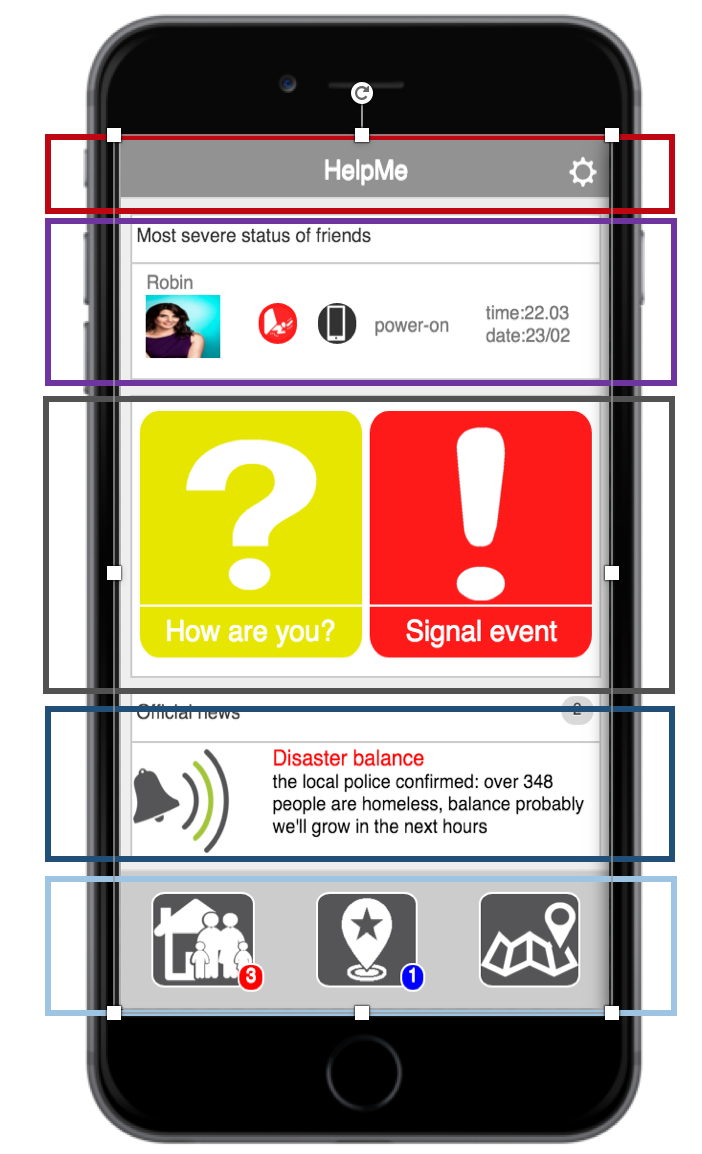
\includegraphics[scale=0.9]{interfaccia/dash.png}
	\caption{Dashboard}
	\label{fig:logo_OSM}
\end{figure}


 
\begin{figure}
\textbf{How are you?:} Per aggiornare il proprio stato bisogna cliccare sul bottone giallo, come in Fig \ref{fig:buttoncomestai}, quindi tappare su un elemento della lista. (Fig \ref{fig:lista}). Per rendere effettivo il nostro aggiornamento basterà cliccare sul tasto in alto a destra:\textit{"Public"}.
\\ \\ \\
 \begin{minipage}[b]{6cm}
   \centering
  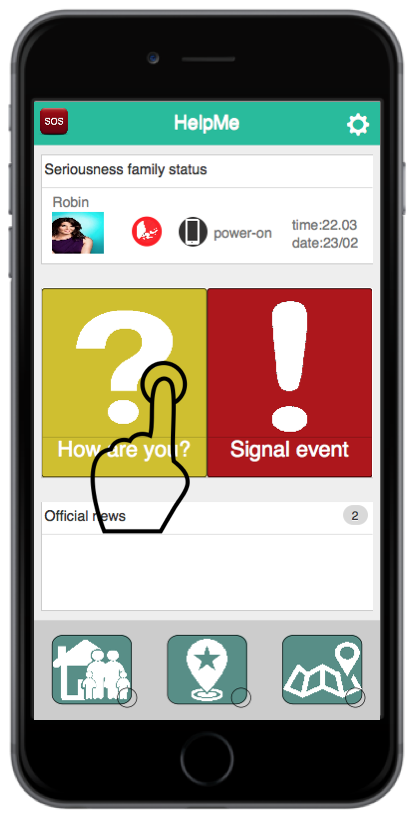
\includegraphics[scale=0.9]{interfaccia/tapbuttoncomestai.png}
	\caption{Tap bottone \textit{"How are you?"}}
	\label{fig:buttoncomestai}
 \end{minipage}
 \ \hspace{6 mm} \hspace{7 mm} \
 \begin{minipage}[b]{6cm}
  \centering
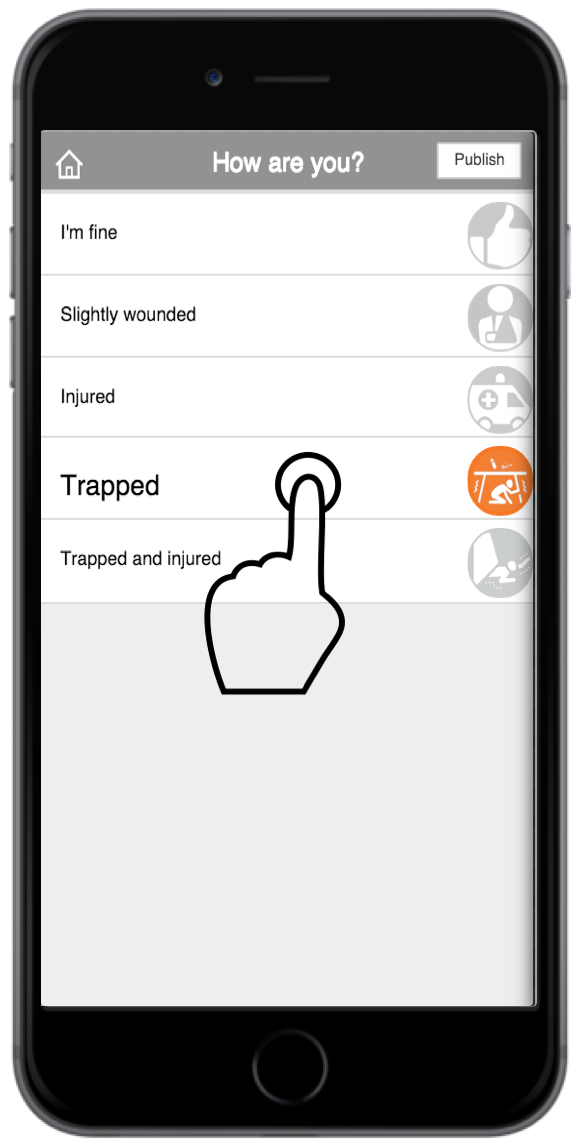
\includegraphics[scale=0.9]{interfaccia/comestaitap.png}
	\caption{Lista predefinita di stati selezionabili}
	\label{fig:lista}
 \end{minipage}
\end{figure}

\newpage


 \begin{figure}
  \textbf{Signal event:} Per segnalare un'emergenza bisogna cliccare, nella dashboard, sul bottone rosso come in Fig \ref{fig:buttonsegnala}, come per gli stati possiamo scegliere l'emergenza da segnalare da una lista predefinita( Fig \ref{fig:lista-em}).
 \\ \\
 \begin{minipage}[b]{6cm}
   \centering
 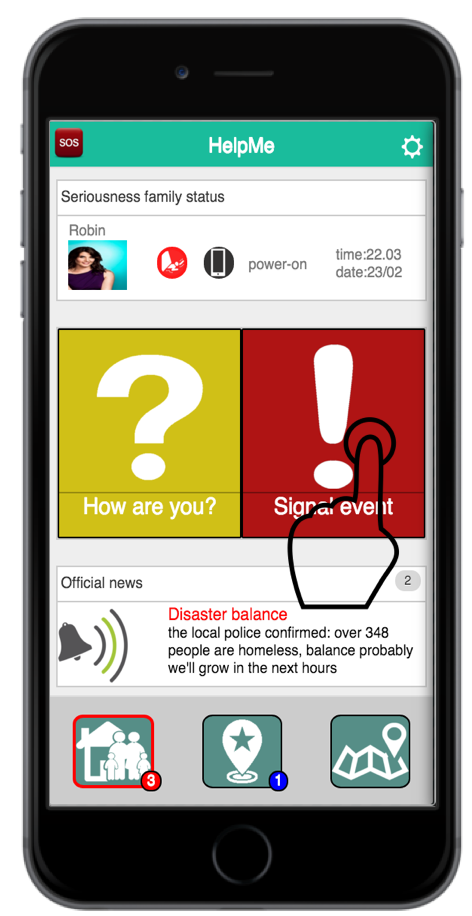
\includegraphics[scale=0.9]{interfaccia/tapbuttonsegnala.png}
	\caption{Tap del bottone \textit{"Signal event"}}
	\label{fig:buttonsegnala}
 \end{minipage}
 \ \hspace{6 mm} \hspace{7 mm} \
 \begin{minipage}[b]{6cm}
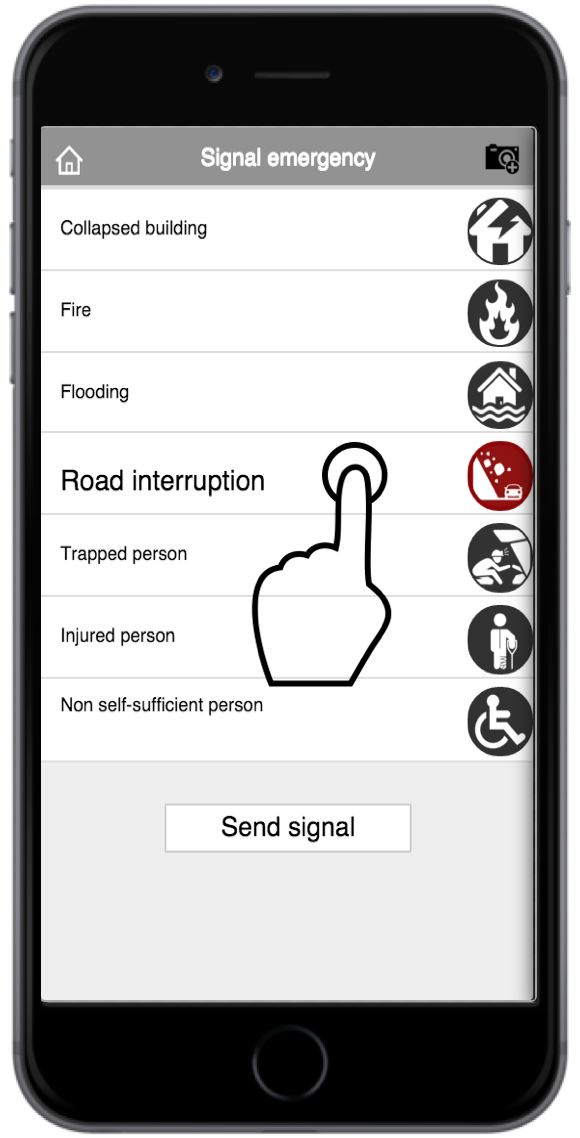
\includegraphics[scale=0.9]{interfaccia/segnalatap.png}
	\caption{Lista predefinita dell'emergenze}
	\label{fig:lista-em}
	
 \end{minipage}
 \\ \\ \\
Quindi premendo sul bottone \textit{"Send signal"}, avremo la possibilità di usare la nostra posizione oppure di utilizzare la mappa (Fig \ref{fig:sceltamappa}).
\end{figure}




 \begin{figure}
\textbf{Where?:} se si decide di utilizzare la mappa per segnalare la posizione, tappando come in Fig \ref{fig:sceltamappa}, allora si dovrà cliccare su un punto della mappa che il sistema ci mostrerà (Fig \ref{fig:mappa-segnala}).
 \\ \\
 \begin{minipage}[b]{6cm}
   \centering
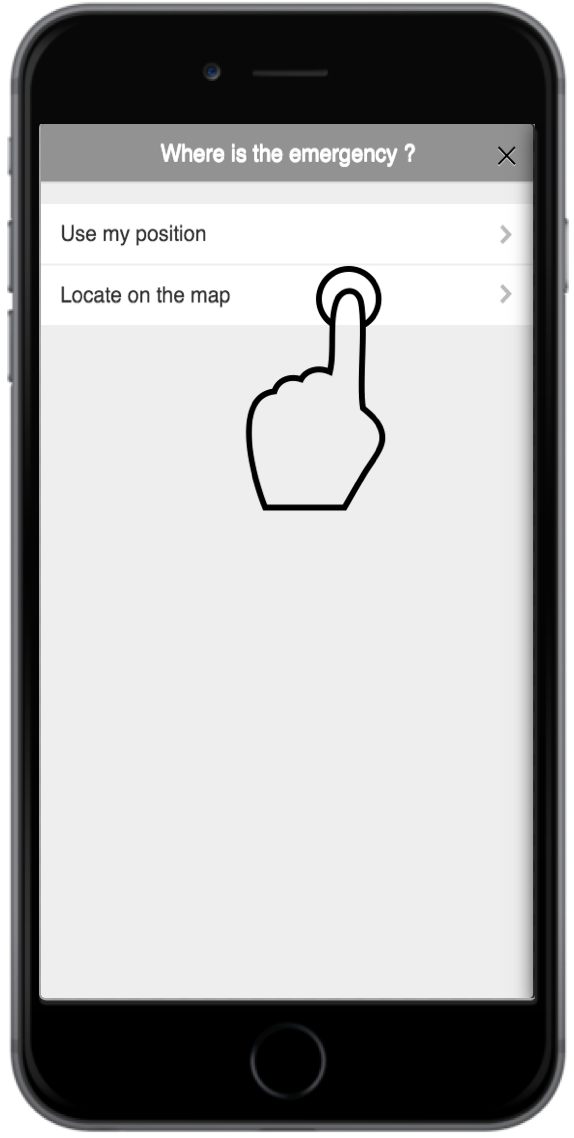
\includegraphics[scale=0.9]{interfaccia/sceltamap.png}
	\caption{Tap \textit{"locate on the map"} }
	\label{fig:sceltamappa}
 \end{minipage}
 \ \hspace{6 mm} \hspace{7 mm} \
 \begin{minipage}[b]{6cm}
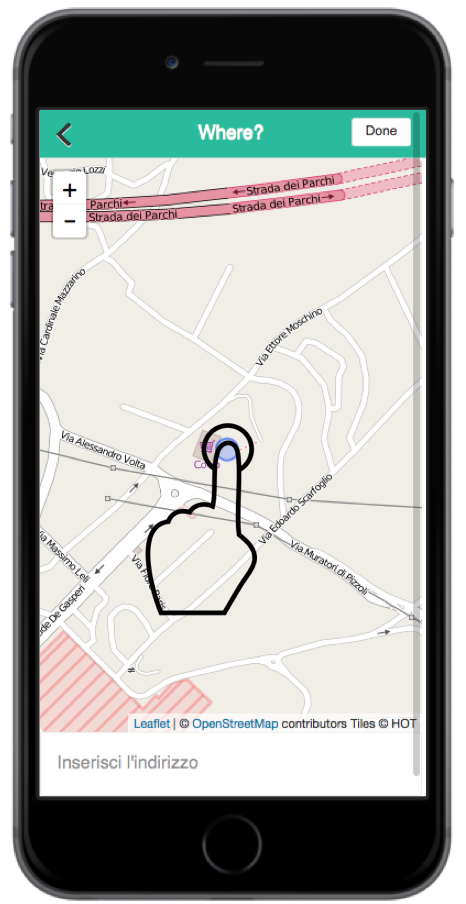
\includegraphics[scale=0.9]{interfaccia/mappasegnala.png}
	\caption{Mappa mostrata dal sistema }
	\label{fig:mappa-segnala}
	
 \end{minipage}
 \\ \\ \\
Per confermare la posizione scelta, basterà cliccare sul tasto \textit{"Done"} e segnalare così l'emergenza. 
\end{figure}



 \begin{figure}
\textbf{Visualizza FOI:} per visualizzare lo stato dei nostri cari bisogna tappare, nella schermata della dashboard, il bottone in basso a sinistra come in Fig \ref{fig:tapfoi}, ottenendo una lista (Fig \ref{fig:lista-foi}) di essi. Questa sarà ordinata per default in base alla gravità del loro stato.
 \\ \\
 \begin{minipage}[b]{6cm}
   \centering
	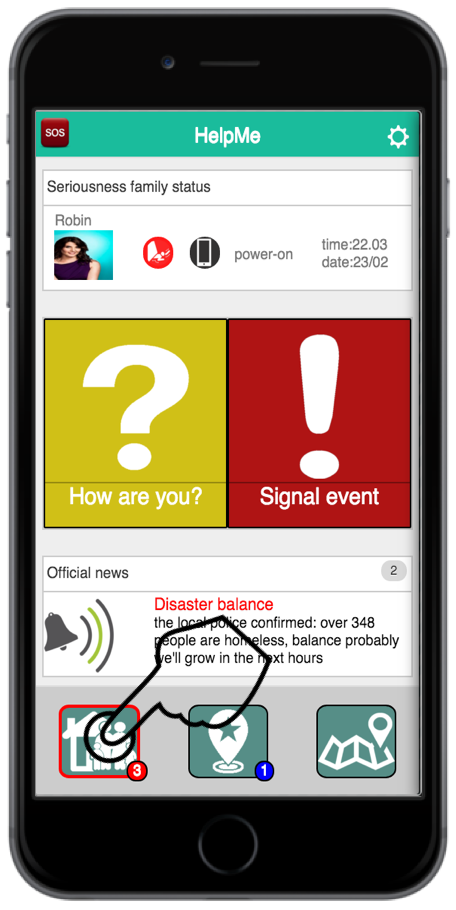
\includegraphics[scale=0.9]{interfaccia/tapfoi.png}
	\caption{Tap da fare per accedere alla lista dei FOI }
	\label{fig:tapfoi}
 \end{minipage}
 \ \hspace{6 mm} \hspace{7 mm} \
 \begin{minipage}[b]{6cm}
\centering
	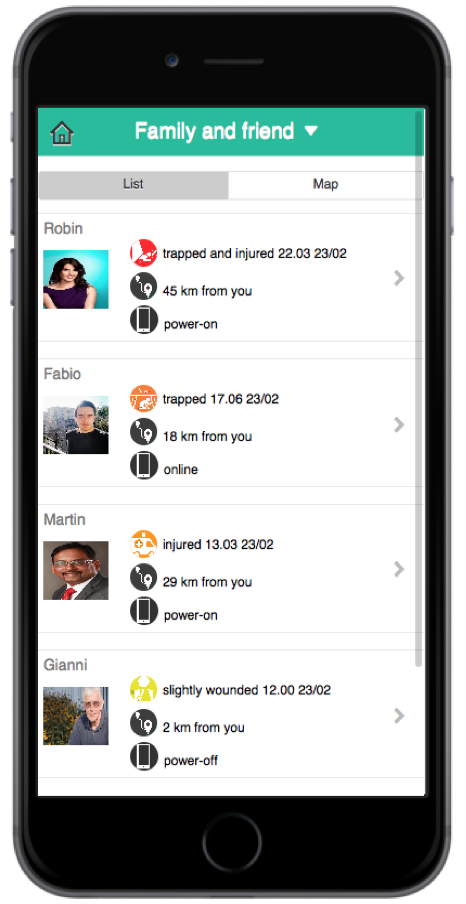
\includegraphics[scale=0.9]{interfaccia/listafoi.png}
	\caption{Lista dei FOI ordinata per default in base alla gravità }
	\label{fig:lista-foi}
 \end{minipage}
\end{figure}


 \begin{figure}
 \textbf{Ordina FOI:} come detto, la lista dei nostri FOI sarà ordinata inizialmente in base alla gravità del loro stato, tuttavia è possibile ordinarla anche a seconda della vicinanza o del più recente aggiornamento semplicemente cliccando prima sull'icona del menu a comparsa, Fig \ref{fig:comparsa}, poi sulla relativa etichetta (Fig \ref{fig:etichetta}).
 \\ \\
 \begin{minipage}[b]{6cm}
   \centering
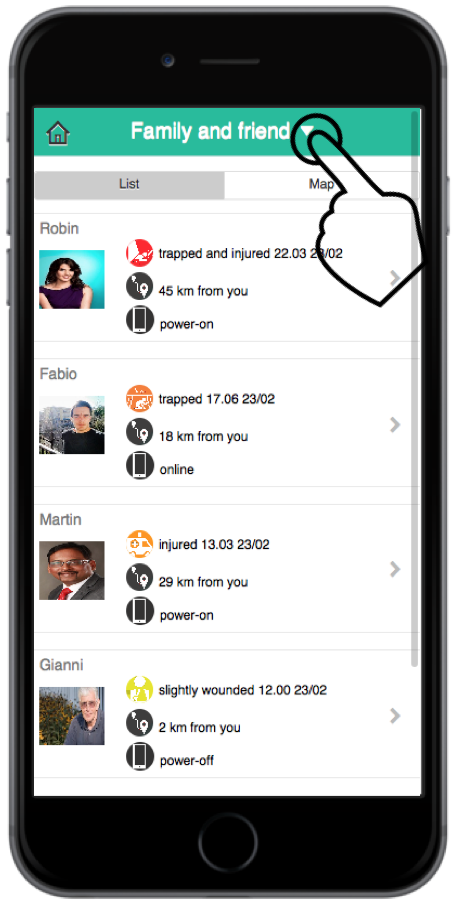
\includegraphics[scale=0.9]{interfaccia/comparsa.png}
	\caption{Tap per aprire il menu a comparsa }
	\label{fig:comparsa}
 \end{minipage}
 \ \hspace{6 mm} \hspace{7 mm} \
 \begin{minipage}[b]{6cm}
\centering
	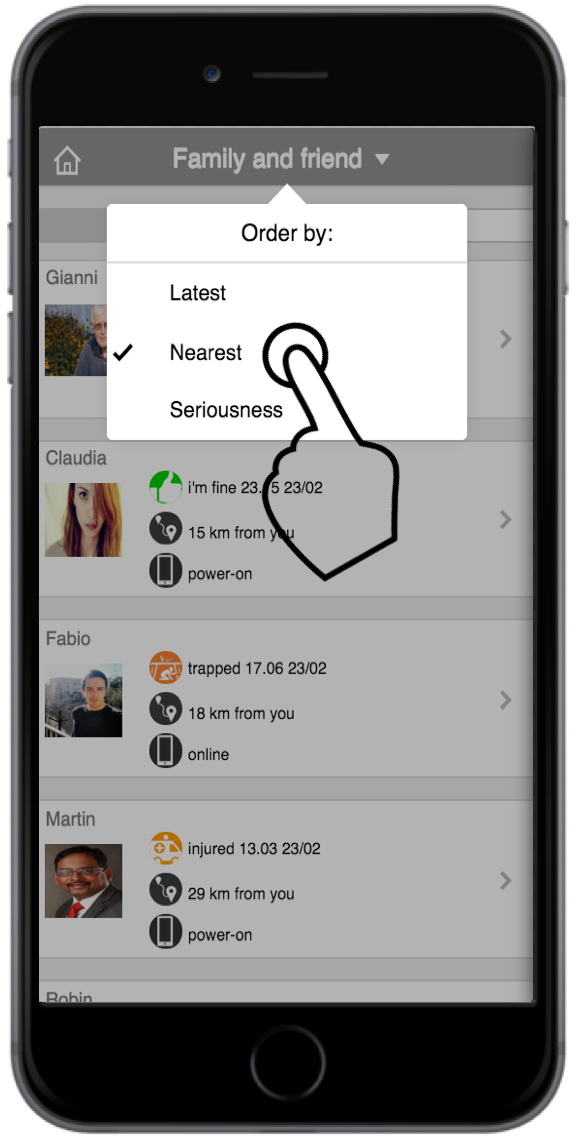
\includegraphics[scale=0.9]{interfaccia/etichetta.png}
	\caption{Tap da fare per ordinare la lista secondo i tre parametri }
	\label{fig:etichetta}
 \end{minipage}
\end{figure}

 \begin{figure}
 \textbf{Visualizza FOI sulla mappa:} oltre alla lista, è possibile visualizzare i propri FOI sulla mappa. Nella schermata precedente basta cliccare sul bottone \textit{"Map"}, come in Fig \ref{fig:mapfoi}.\\
 La mappa verrà centrata sul primo foi della lista e quindi in base all'ordinamento di essa, nell'esempio di Fig \ref{fig:mappafoi}, la mappa era ordinata per vicinanza.
 \\ \\
 \begin{minipage}[b]{6cm}
   \centering
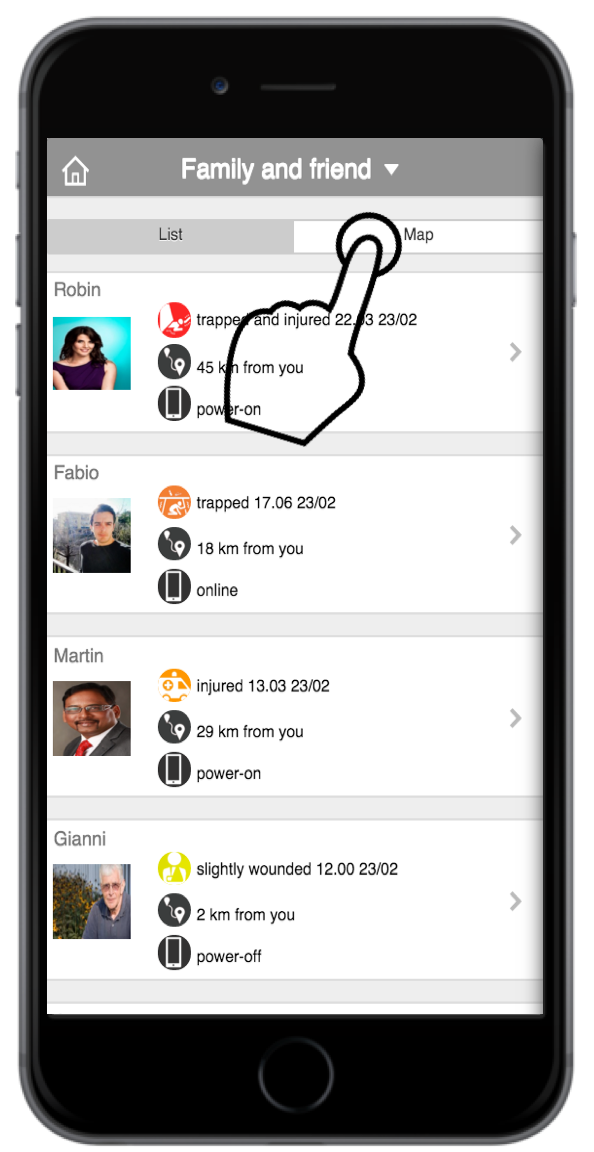
\includegraphics[scale=0.9]{interfaccia/mapfoi.png}
	\caption{Tap per visualizzare i FOI sulla mappa }
	\label{fig:mapfoi}
 \end{minipage}
 \ \hspace{6 mm} \hspace{7 mm} \
 \begin{minipage}[b]{6cm}
\centering
	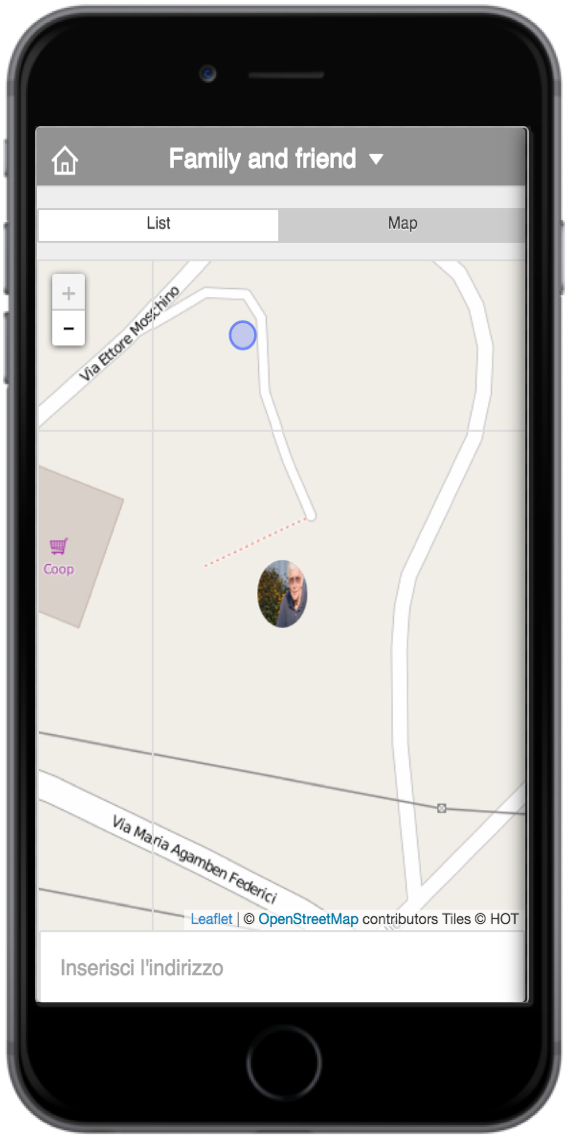
\includegraphics[scale=0.9]{interfaccia/mappafoi.png}
	\caption{Mappa centrata sul FOI più vicino }
	\label{fig:mappafoi}
 \end{minipage}
 \\ \\
E' possibile comunque, con le stesse modalità della lista, centrare la visuale della mappa in base al FOI più vicino, più grave o che abbia aggiornato più recentemente il suo stato
\end{figure}



 \begin{figure}
 \textbf{Clustermarker FOI:} come specificato nei requisiti, i marker dei FOI (e dei POI) devono essere raggruppati quando lo zoom della mappa è tale da farli "toccare" (Fig \ref{fig:markercluster}).\\
Inoltre cliccando il clustermarker è possibile vedere da quali FOI è composto (Fig \ref{fig:markerfoi}). 
 \\ \\
 \begin{minipage}[b]{6cm}
   \centering
	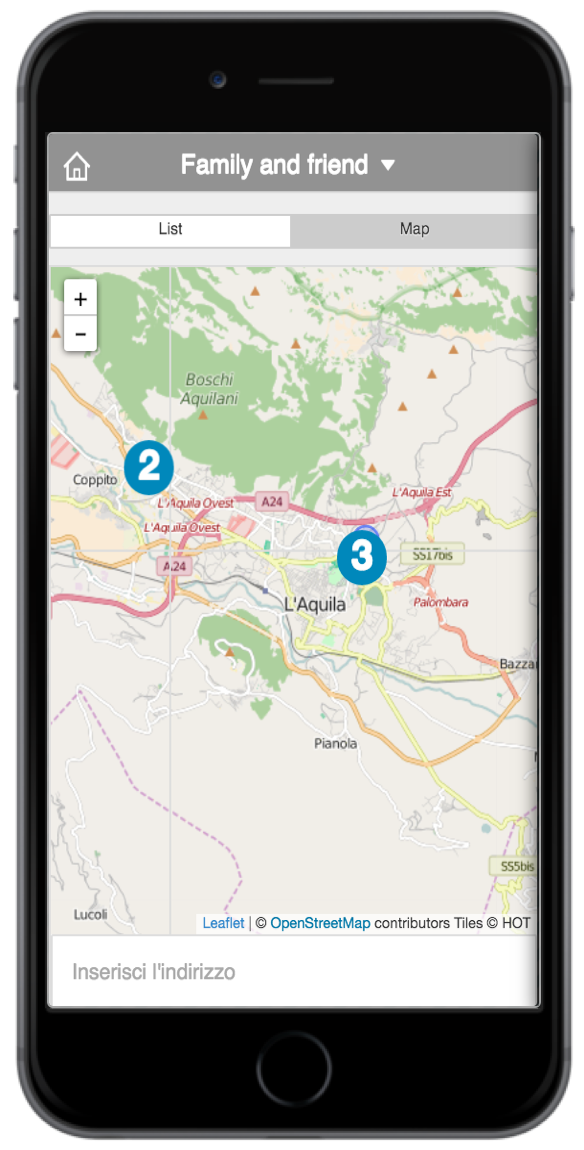
\includegraphics[scale=0.9]{interfaccia/markercluster.png}
	\caption{Due markercluster contenenti rispettivamente due e tre FOI }
	\label{fig:markercluster}
 \end{minipage}
 \ \hspace{6 mm} \hspace{7 mm} \
 \begin{minipage}[b]{6cm}
\centering
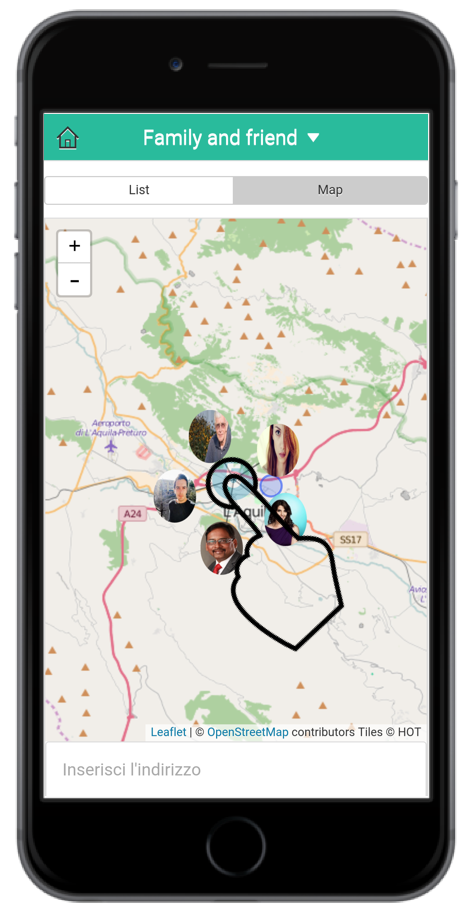
\includegraphics[scale=0.9]{interfaccia/markerfoi.png}
	\caption{Tap su un markercluster contenente cinque FOI }
	\label{fig:markerfoi}
 \end{minipage}
\end{figure}

 \begin{figure}
\textbf{ POI:} le modalità di interazione e le schermate sono analoghe a quelle viste per i FOI. \\
Dalla dashboard bisogna cliccare sul bottone in fondo, come mostrato in Fig \ref{fig:buttonpoi}, per accedere alla lista (Fig \ref{fig:poilist}).
 \\ \\
 \begin{minipage}[b]{6cm}
   \centering
	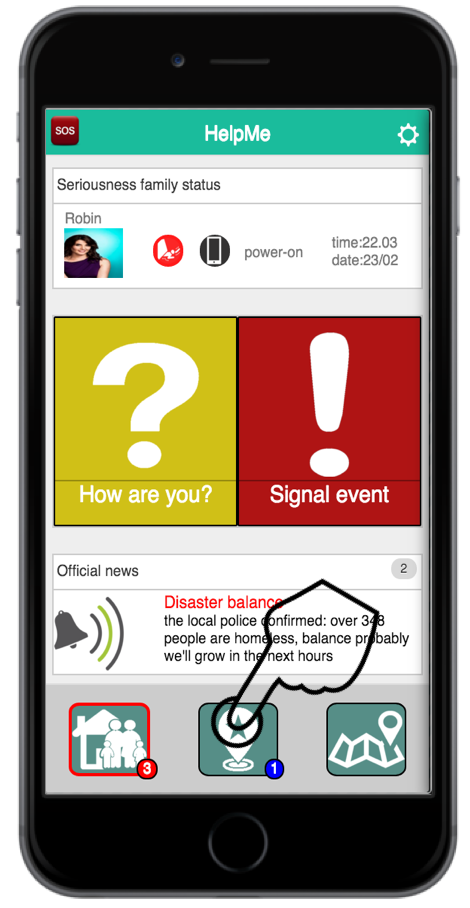
\includegraphics[scale=0.9]{interfaccia/buttonpoi.png}
	\caption{Tap da fare per accedere ai propri POI }
	\label{fig:buttonpoi}
 \end{minipage}
 \ \hspace{6 mm} \hspace{7 mm} \
 \begin{minipage}[b]{6cm}
\centering
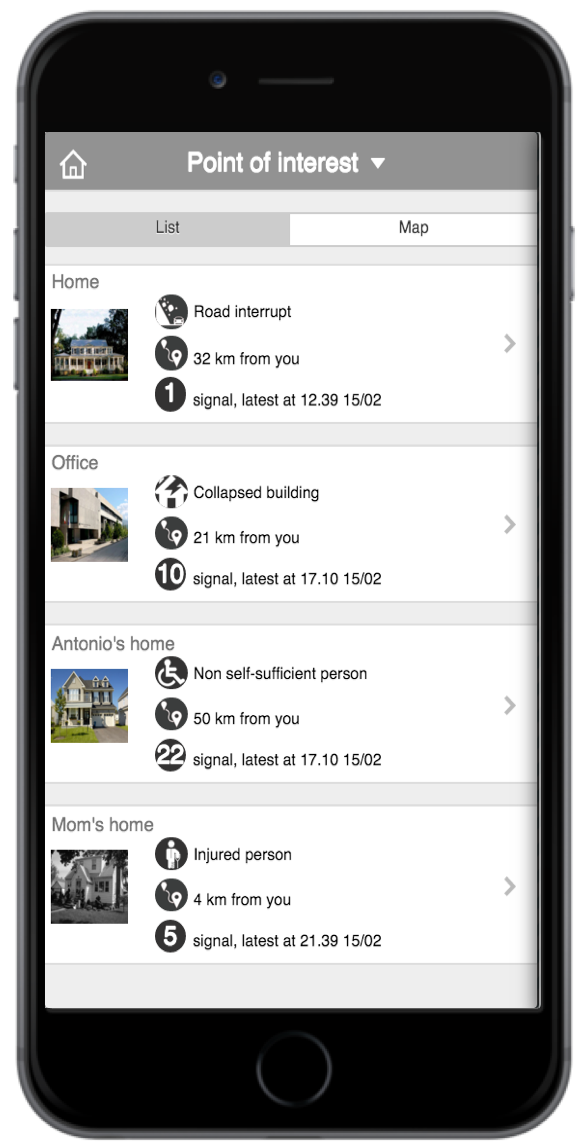
\includegraphics[scale=0.9]{interfaccia/poilist.png}
	\caption{Lista dei POI ordinata per default in base al più recente }
	\label{fig:poilist}
 \end{minipage}
\end{figure}

 \begin{figure}
\textbf{ POI:} le modalità di interazione e le schermate sono analoghe a quelle viste per i FOI. Inoltre tappando su un generico marker, è possibile visualizzare il relativo stato e l'ora in cui è stato aggiornato (Fig \ref{fig:tapmarker}). 
 \\ \\
 \begin{minipage}[b]{6cm}
   \centering
	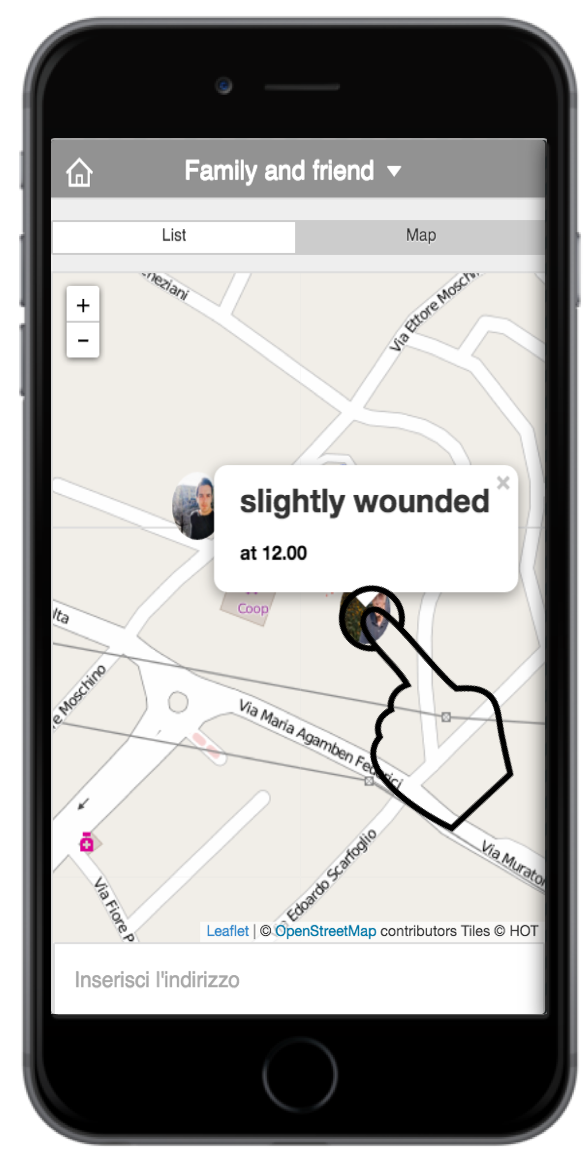
\includegraphics[scale=0.9]{interfaccia/tapmarker.png}
	\caption{Tap sul marker del FOI }
	\label{fig:tapmarker}
 \end{minipage}
 \ \hspace{6 mm} \hspace{7 mm} \
 \begin{minipage}[b]{6cm}
\centering
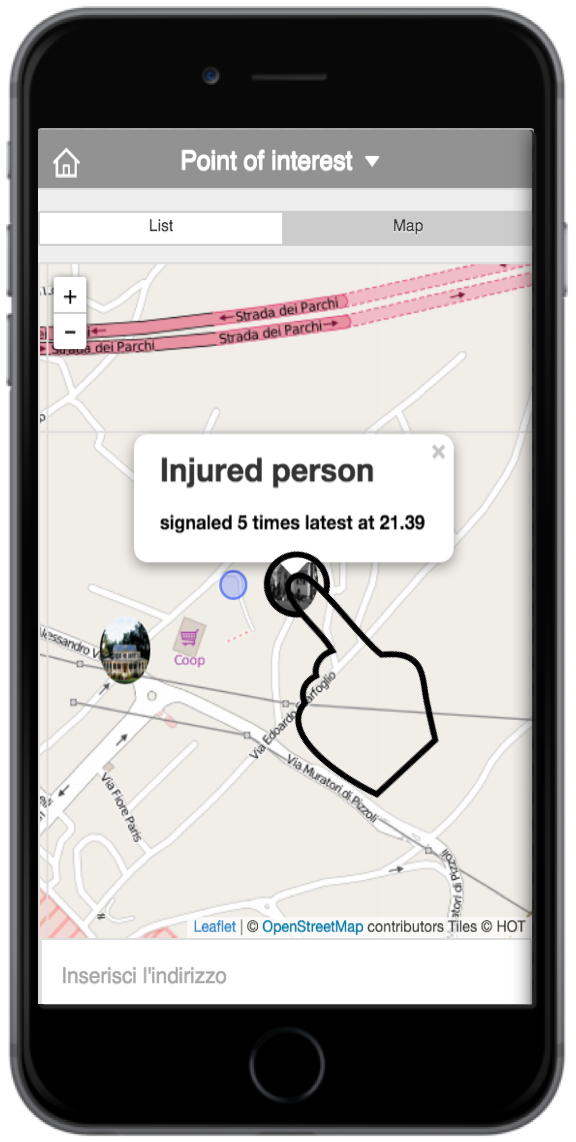
\includegraphics[scale=0.9]{interfaccia/tappoimarker.png}
	\caption{Tap sul marker di un POI }
	\label{fig:poilist}
 \end{minipage}
\end{figure}





	